\section{ SR01BR15 }


\subsection{Meta}

    \textbf{Title:}
    Solutions in radiology services management: a literature review

    \begin{table}[H]
        \centering
        \begin{tabular}{|c|c|c|c|c|c|c|c|c|}
            \hline
                \textbf{Rank} & \textbf{Grasp} & \textbf{Grade} & \textbf{Type} & \textbf{Outcome} & \textbf{Domain} & \textbf{COV19} & \textbf{CoI} & \textbf{DB} \\
            \hline
                0 & 98\% & E & A & ?? & ?? & No & ?? & No \\
            \hline
        \end{tabular}
        \caption{Reference's metadata}
        \label{tab:SR01BR15}
    \end{table}

\subsection{Summary}
    Aline Garcia Pereira et al. \cite{x073} rendered qualitative research on the issues in radiology (presumably in Brazil). This literature review covered various topics in general terms and proposes some solutions. On the other hand, the quality of the work and the issues that arose in the research show that the situation in the field of radiology in Brazil until 2014 was critical. The phrase "procedure scheduling" in the abstract of this work is misleading. Hence, there is no discussion of the radiology procedure scheduling, meaning that this work is outside the scope of our literature review. A few things in this study could have value: mentioning the no-shows, latency to radiological appointments and the critical situation with radiology in Brazil. 

\subsection{Notes}
    \begin{itemize}
        \item Scopus, SciELO, Mendeley;
        \item Communication with patients through Facebook and Twitter;
        \item "5S" principles?
    \end{itemize}


\subsection{Reading}
    \textbf{Abstract:}
    General, qualitative overview of the problems in radiological department.
    
    \textbf{Objectives:}
    Review existig issues with radiology services: “to develop hypotheses; increase investigators’ awareness of a given environ- ment, fact or phenomenon, in order to further and more ac- curately investigate in the future, or to modify and clarify concepts”
    
    \textbf{Page 1 (Introduction):}
    History and introduction to X-rays in healthcare perspective. There are healthcare problems in Brazil. To solve these problems the authors adress the need for quality control, radioprotection, biosafety, humanization, and new technology. This literature review contains overviews on buplications from 1982 to 2014 and is not limited just to articles. 
    
    \textbf{Page 2 (Materials and Methods):}
    Here the authors outline the methodolody, methods, and tools used for the literature review.
    
    \begin{figure}[H]
        \centering
        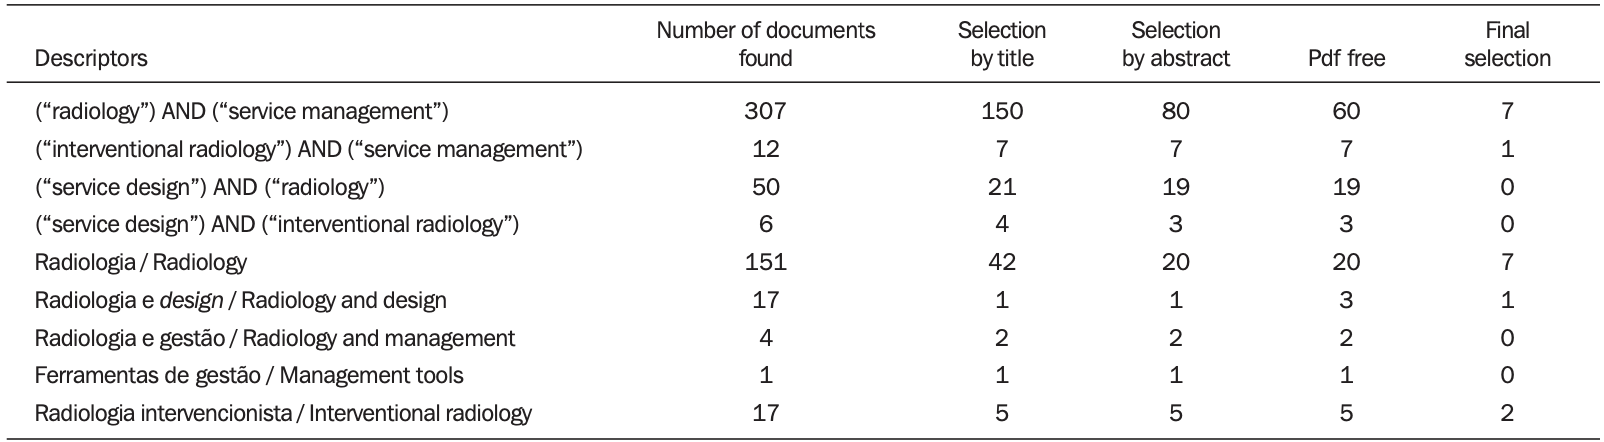
\includegraphics[width=.7\textwidth]{figures/0016_SR01BR15/fig1.png}
        \caption{Queries to Scopus and SciELO databases in \cite{x073}.}
        \label{fig1:0016_SR01BR15}
    \end{figure}
    
    \textbf{Page 3 (Results):}
    Just general info about the importance of considering humans as main objectives in the hospital management. \underline{Waiting time and problems with appointment scheduling}: Uncertainty prediction; patient classification; no-show rescheduling. \underline{Interaction with users}: Implementation of social media for two-side communication with the patients shows some valuable results on practice... 

    \textbf{Page 4 (Results):}
    ... \underline{Equipment and tests}: some discussions and examples of available radiology equipment. \underline{Multidisciplinary knowledge}: The medical personnel require more education to handle the radiology equipment to protect themselves and the patients from excessive radiation. \underline{Management}: safety rules + staff interaction guidance + personnel-patient interaction guidance.

    \textbf{Page 5 (Discussion):}
    Repeating general staff about the management definition, enterprice-personnel cooperation, radiology workplace safety.
    
    \textbf{Page 6 (Conclusion):}
    Patients in the focus. Small number of articles in the radiology. Improve the level of education for healthcare professionals. Learn to implement knowledge on practice.